\documentclass[UTF8]{ctexart}
\title{第七章 设计结果验证}
\author{陈登}
\date{\today}

\bibliographystyle{plain}
\usepackage{graphicx}
\usepackage{float}
\usepackage{amsmath}
\usepackage{geometry}
\usepackage{fontspec}
\usepackage{algorithm}
\usepackage{algorithmicx}
\usepackage{algpseudocode}
\usepackage{diagbox}

\geometry{a4paper,centering,scale=0.9}
\usepackage[format=hang,font=small,textfont=it]{caption}
\usepackage[toc,page,title,titletoc,header]{appendix}
\usepackage[nottoc]{tocbibind}

\begin{document}

\section{设计结果验证}

本章节主要根据各个层级的相关设计要求给出具体的各个模块设计仿真、综合结果。

\subsection{接收端数据链路层}

数据链路层主要包含五个部分的模块,8B/10B解码器模块,解扰器模块,码群同步模块,初始化帧同步模块,初始化lane同步模块。

\subsubsection{8B/10B解码器}

\paragraph{仿真}

设计完整功能的8B/10B解码器仿真结果如图\ref{fig:8b_10b_decoder_wave}所示。

\begin{figure}[H]
	\centering
	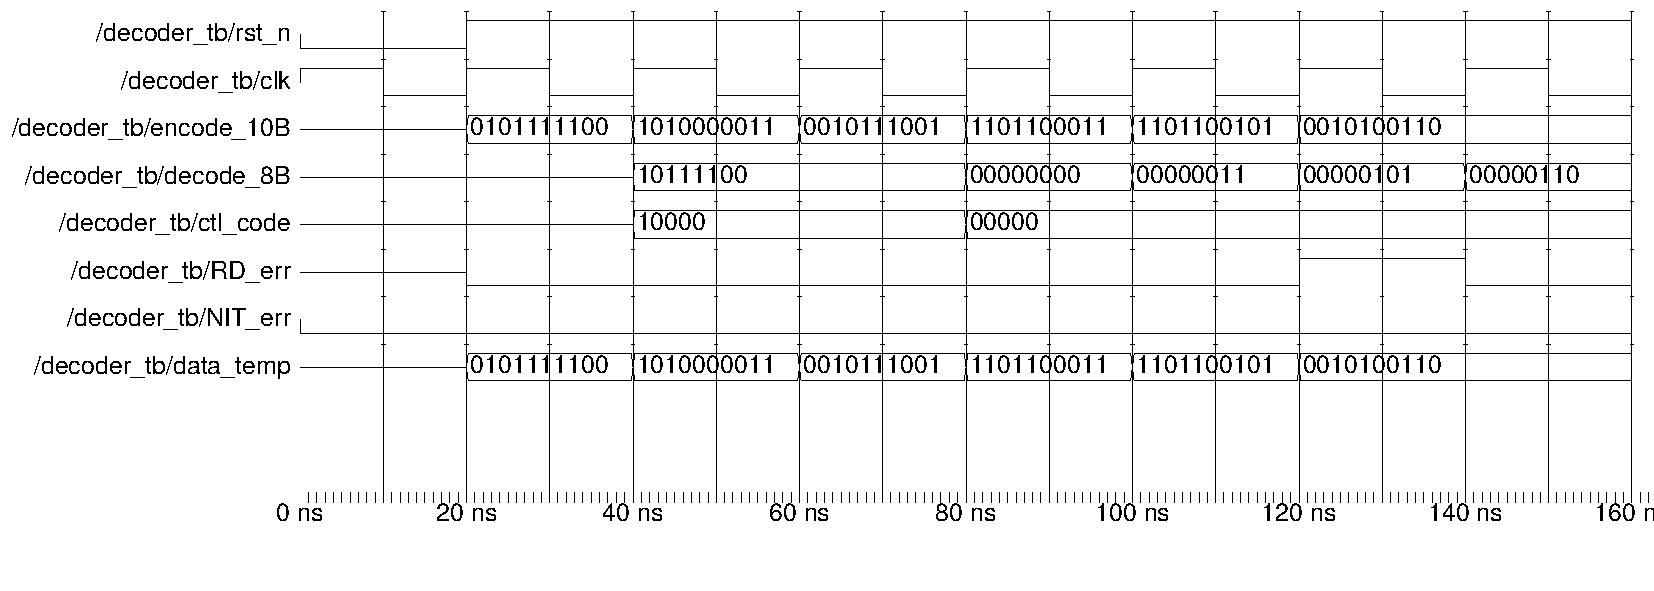
\includegraphics[width=18cm]{./img/8b_10b_decoder_wave.pdf}
	\caption{8B/10B解码器仿真结果}
	\label{fig:8b_10b_decoder_wave}
\end{figure}

可以看到,在复位信号启动后,输入端口收到了一系列的10B数据,并对这10B数据进行解码。
第一个接收到的数据为/K28.5/的10B编码,并且是极性呈正极性。
由于协议规定,8B/10B解码器初始的极性状态规定为负极性,所以最初传入的10B正极性数据并不会引起极性错误。
输入和输出之间由于有处理时延,所以通过时钟划定了一个octet时钟周期的时延。
第一个解码来的字符是/K28.5/,在ctl\_code端口可以看到编码为10000,其中置高的一位即表示/K/控制字符。
由于是控制字符,输出的具体解码数据并不重要。
第二个收到的字符也为/K28.5/的10B编码,不过由于之前一个10B编码表现为正极性,而此次收到的10B编码为负极性,并不会引起极性错误。
第二个字符的解码输出同第一个字符的解码输出,此时接收端极性为负极性。
第三个字符不再是控制字符,而是数据字符/D0.0/并且是一个中性极性的编码,并不改变当前极性,解码输出为00000000,解码正确。
第四个字符是数据字符/D3.0/,这是一个正极性的编码,与本地极性相反所以不会发生极性错误,本地极性翻转为正极性,解码输出为00000011,解码正确。
第五个字符是数据字符/D5.0/,这也是一个正极性的编码,与本地极性相同,所以接收端在此时RD\_err信号置高,表示发生极性错误,本地极性以刚接收到的数据极性为准,保持正极性,解码输出为00000101,解码正确。
由此可见,解码的正确与否与极性是否正确没有直接关系,极性错误并不会直接导致解码错误。
第六个字符是数据字符/D6.0/,这是一个负极性的编码,与本地极性相反,所以没有发生极性错误,解码输出为00000110,解码正确。

在这6个字符的测试序列中基本展示了8B/10B解码器的基本功能,包括了解码、极性错误判断和控制字符判断。
基本功能测试基本已经实现。

\paragraph{综合}

综合过程一般分为四步:设定工艺库、读入RTL设计、进行综合、输出报告。
Linux下的DC可以通过GUI界面和命令行进行综合。
读入设计后可以通过GUI观察详细的门电路级电路,使用的器件既为器件库中所包含的器件。

综合完成后就可以得到详细的综合报告。
比较有价值的即面积报告、时序报告和功耗报告。
其中面积报告可以将每个子模块占用的面积总结出来,单位为平方微米($\mu m^2$);
时序报告会找到耗时最长的路径以表示电路最高的工作速度,单位为纳秒($ns$);
功耗报告即整体的功率损耗,单位为纳瓦($nW$)。

表\ref{tab:tab1_syn_compare}详细比较了几种设计,其中括号里面的比例均为和新设计比较的比例,即视新设计具体之为100\%。

\begin{table}[H]
\centering
\caption{综合具体结果比较}
\label{tab:tab1_syn_compare}
\begin{tabular}{|c|r|r|r|}

\hline

\diagbox{项目}{设计} 			&	Classic 	&	Actel 		&	New 	\\

\hline

RD Cal Area($\mu m^2$)			&				&	665(99\%)	&	675		\\

4B/3B Area($\mu m^2$)			&				&	369(148\%)	&	249		\\

6B/5B Area($\mu m^2$)			&				&	1184(172\%)	&	688		\\

\hline

Sum Area($\mu m^2$)				&	1570(97\%)	&	2218(138\%)	&	1612	\\

\hline

Total Cell Area($\mu m^2$)		&	1716(98\%)	&	2657(151\%)	&	1759	\\

\hline

Total Area($\mu m$)				&	16836(107\%)&	24497(156\%)&	15666	\\

\hline

Timing($ns$)					&	8.16 		&	9.97		&	9.54 	\\

Time Used($ns$)					&	5.84		&	4.03		&	4.46	\\

\hline

Frequency($MHz$)				&	171.2(76\%)	&	248.1(111\%)&	224.2 	\\

\hline

Cell Internal Power($nW$)		&	22.6(83\%)	&	31.0(114\%)	&	27.2 	\\

Net Switing Power($nW$)			&	42.8(80\%)	&	50.1(94\%)	&	53.3 	\\

\hline

Total Dynamic Power($nW$)		&	65.4(81\%)	&	81.1(101\%)	&	80.5 	\\

\hline

\end{tabular}
\end{table}

相较于Actel方法,新设计在频率上有11\%的减少,但是在面积上,无论是单元面积还是总面积都减少了近50\%的提升。
两者在功耗上几乎相同。
相较于传统方法,新设计在频率上有近25\%的提升,在单元面积上几乎相同,在总面积上减少了7\%。
但是在功耗上有近20\%的差距。


\subsubsection{解扰器}

\subsubsection{码群同步}

\subsubsection{初始化帧同步}

\subsubsection{初始化lane同步}

\subsection{接收端传输层}

\subsubsection{解帧器}

\subsection{确定性时延}

\subsubsection{接收缓冲}

\subsubsection{Subclass 1类设备本地多帧时钟对齐}

\subsubsection{Subclass 2类设备本地多帧时钟对齐}

\bibliography{../../bib/serdes}
\end{document}
